% 数据图 include 片段（19 张 DATA 图，全部为矢量 PDF）
% 用法：正文 \input 本文件对应段落，或直接复制单个 figure 环境。
% 需要的宏包：graphicx、float。图片路径以论文主文件所在目录为基准，
% 若主文件不在仓库根目录，请调整 \graphicspath 或下面的相对路径。
% caption 均为 ≤20 字的中文名词短语；统计口径、数据来源与结论请写在正文，
% 不要搬进 \caption{}。

% ==== 数据处理 ============================================================
\begin{figure}[H]
  \centering
  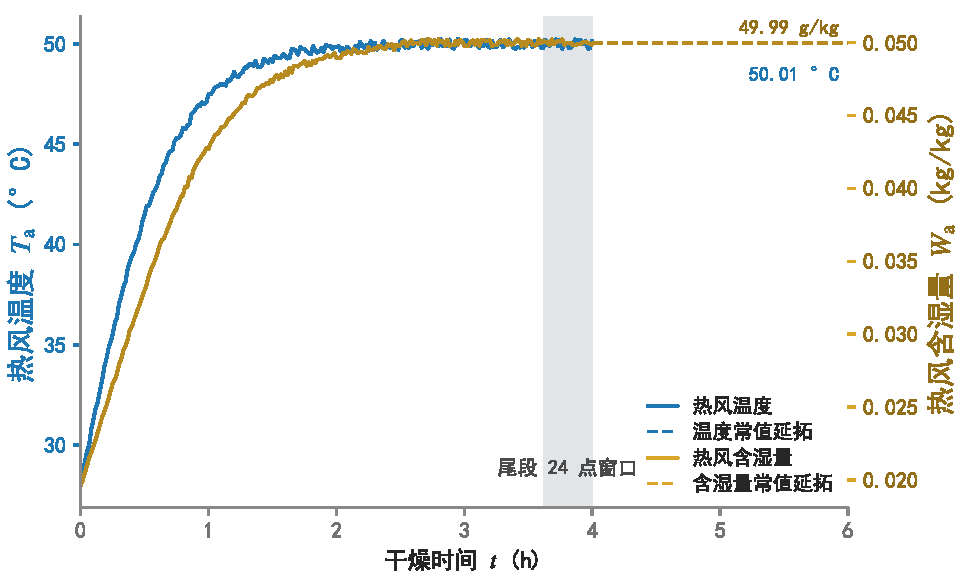
\includegraphics[width=0.9\textwidth,height=0.8\textheight,keepaspectratio]{figures/fig_air_condition.pdf}
  \caption{热风温度与含湿量时程}
  \label{fig:air_condition}
\end{figure}

\begin{figure}[H]
  \centering
  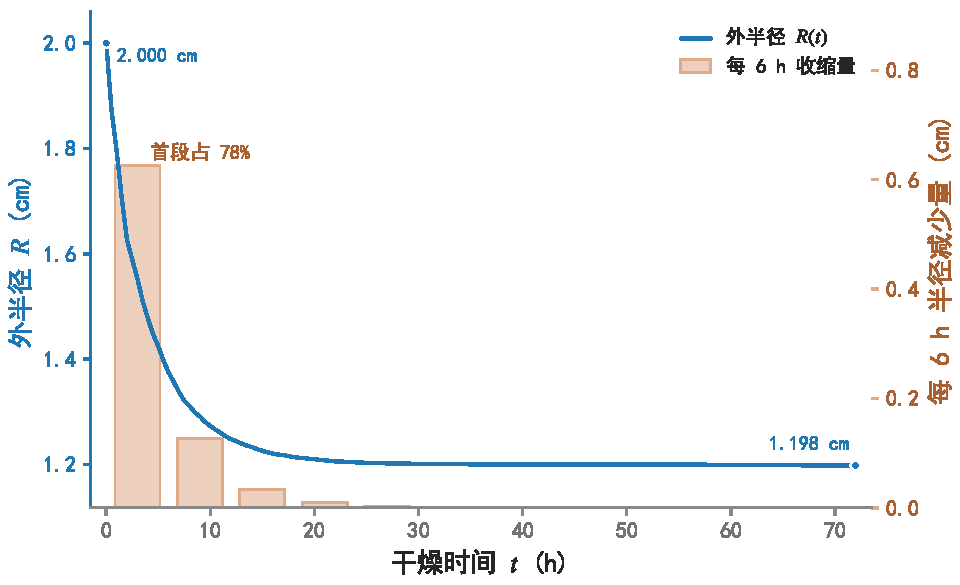
\includegraphics[width=0.9\textwidth,height=0.8\textheight,keepaspectratio]{figures/fig_shrinkage_curve.pdf}
  \caption{药材半径收缩曲线}
  \label{fig:shrinkage_curve}
\end{figure}

% ==== 问题一 ==============================================================
\begin{figure}[H]
  \centering
  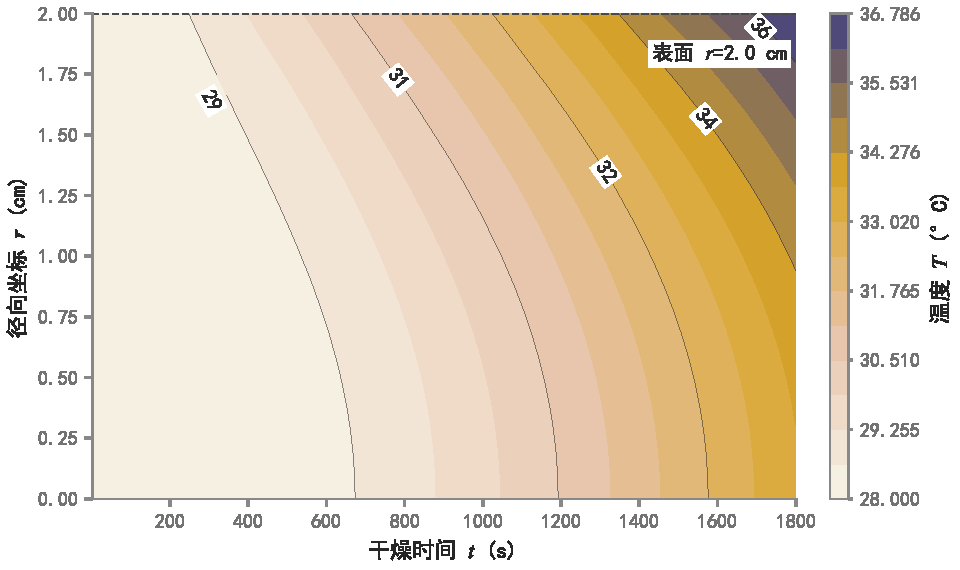
\includegraphics[width=0.9\textwidth,height=0.8\textheight,keepaspectratio]{figures/fig_q1_field_T.pdf}
  \caption{问题一温度场分布}
  \label{fig:q1_field_T}
\end{figure}

\begin{figure}[H]
  \centering
  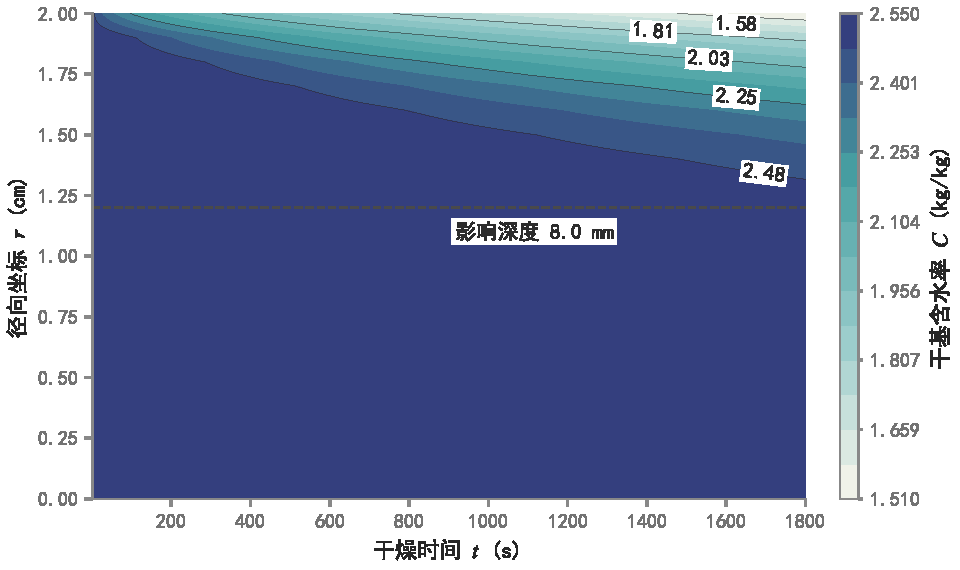
\includegraphics[width=0.9\textwidth,height=0.8\textheight,keepaspectratio]{figures/fig_q1_field_C.pdf}
  \caption{问题一含水率场分布}
  \label{fig:q1_field_C}
\end{figure}

\begin{figure}[H]
  \centering
  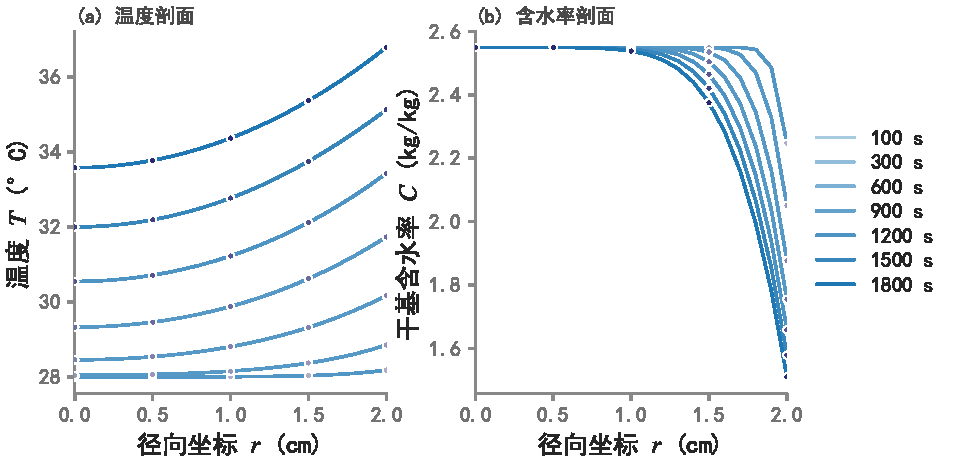
\includegraphics[width=0.9\textwidth,height=0.8\textheight,keepaspectratio]{figures/fig_q1_profiles.pdf}
  \caption{问题一径向剖面族}
  \label{fig:q1_profiles}
\end{figure}

\begin{figure}[H]
  \centering
  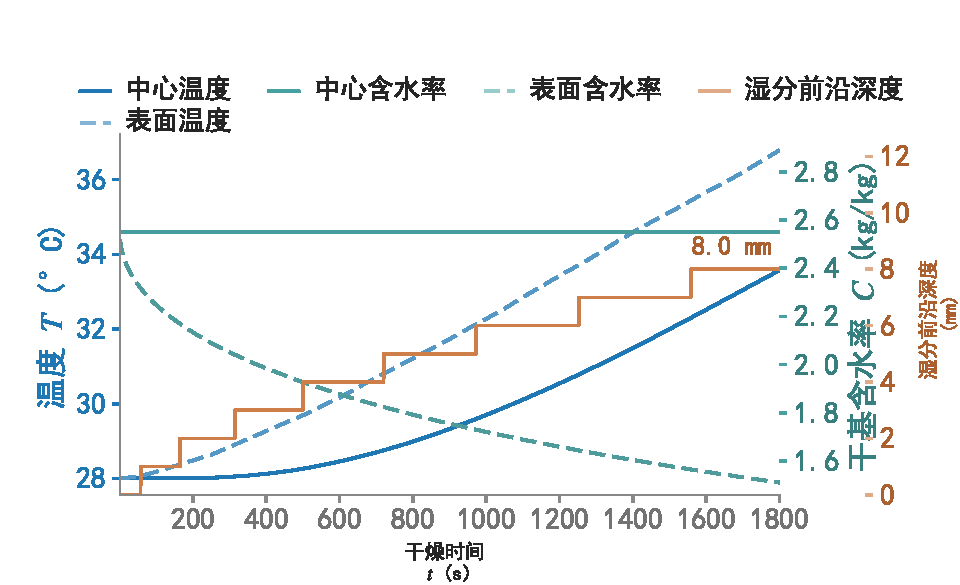
\includegraphics[width=0.9\textwidth,height=0.8\textheight,keepaspectratio]{figures/fig_q1_penetration.pdf}
  \caption{问题一热湿推进对比}
  \label{fig:q1_penetration}
\end{figure}

% ==== 问题二 ==============================================================
\begin{figure}[H]
  \centering
  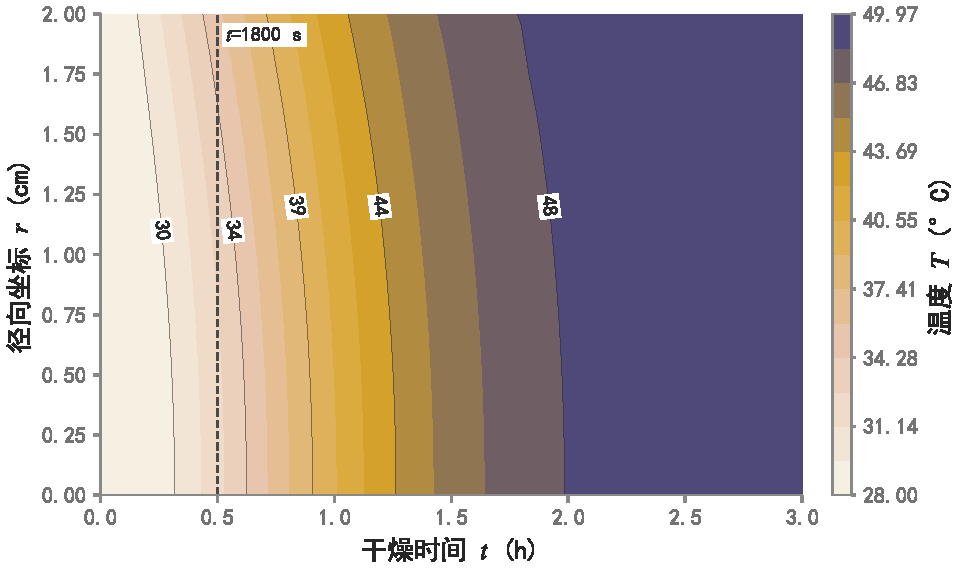
\includegraphics[width=0.9\textwidth,height=0.8\textheight,keepaspectratio]{figures/fig_q2_field_T.pdf}
  \caption{问题二温度场分布}
  \label{fig:q2_field_T}
\end{figure}

\begin{figure}[H]
  \centering
  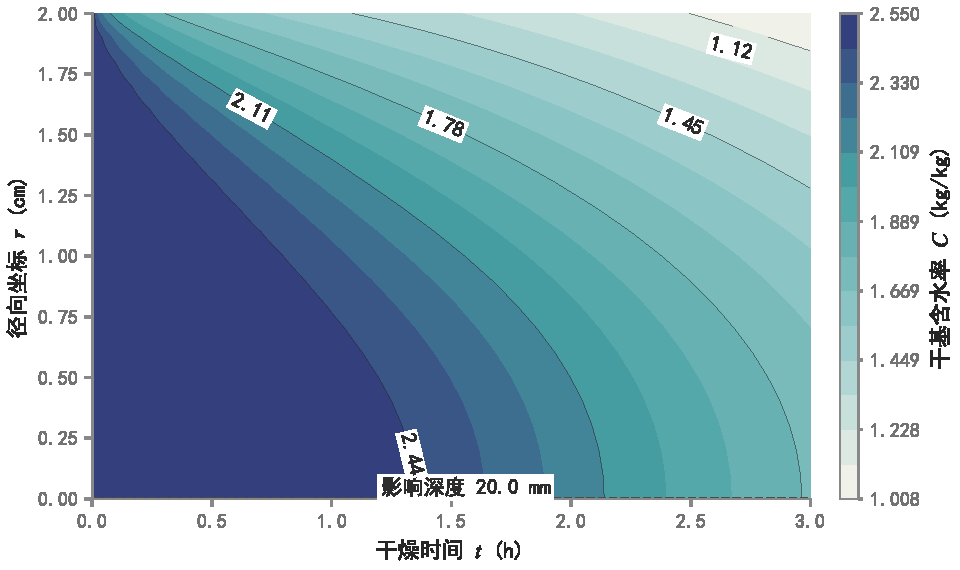
\includegraphics[width=0.9\textwidth,height=0.8\textheight,keepaspectratio]{figures/fig_q2_field_C.pdf}
  \caption{问题二含水率场分布}
  \label{fig:q2_field_C}
\end{figure}

\begin{figure}[H]
  \centering
  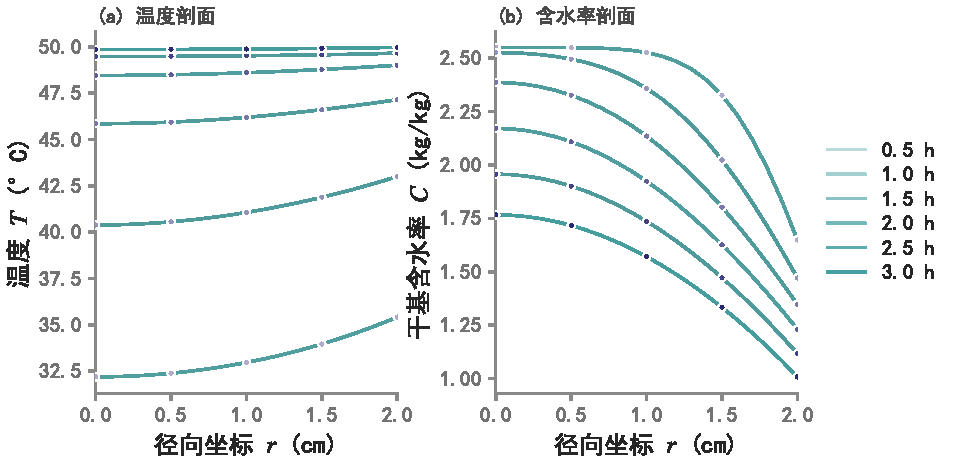
\includegraphics[width=0.9\textwidth,height=0.8\textheight,keepaspectratio]{figures/fig_q2_profiles.pdf}
  \caption{问题二径向剖面族}
  \label{fig:q2_profiles}
\end{figure}

\begin{figure}[H]
  \centering
  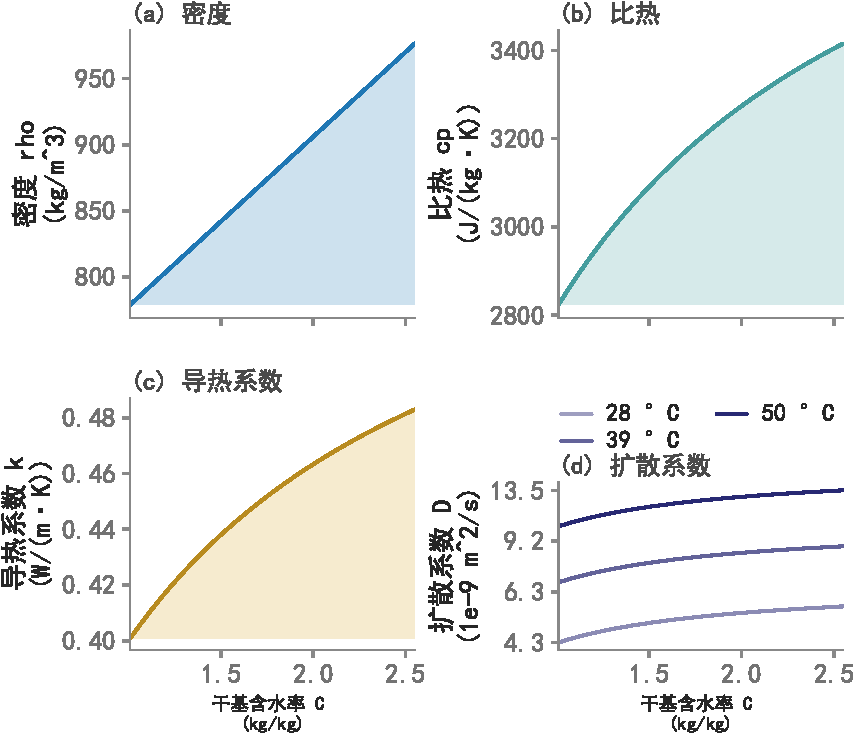
\includegraphics[width=0.8\textwidth,height=0.8\textheight,keepaspectratio]{figures/fig_q2_props_evolution.pdf}
  \caption{附录三物性随含水率变化}
  \label{fig:q2_props_evolution}
\end{figure}

\begin{figure}[H]
  \centering
  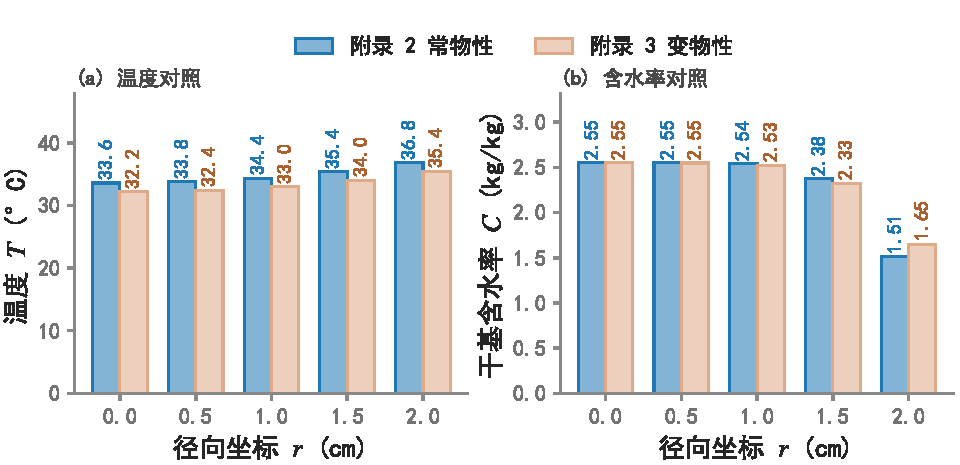
\includegraphics[width=0.9\textwidth,height=0.8\textheight,keepaspectratio]{figures/fig_q1q2_contrast.pdf}
  \caption{常物性与变物性结果对照}
  \label{fig:q1q2_contrast}
\end{figure}

% ==== 问题三 ==============================================================
\begin{figure}[H]
  \centering
  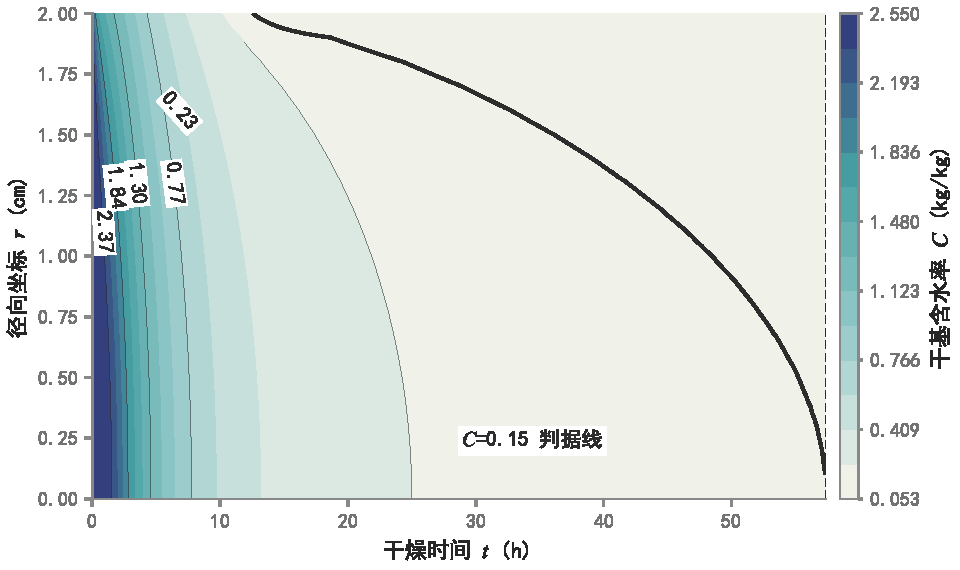
\includegraphics[width=0.9\textwidth,height=0.8\textheight,keepaspectratio]{figures/fig_q3_field_C.pdf}
  \caption{问题三全程含水率场}
  \label{fig:q3_field_C}
\end{figure}

\begin{figure}[H]
  \centering
  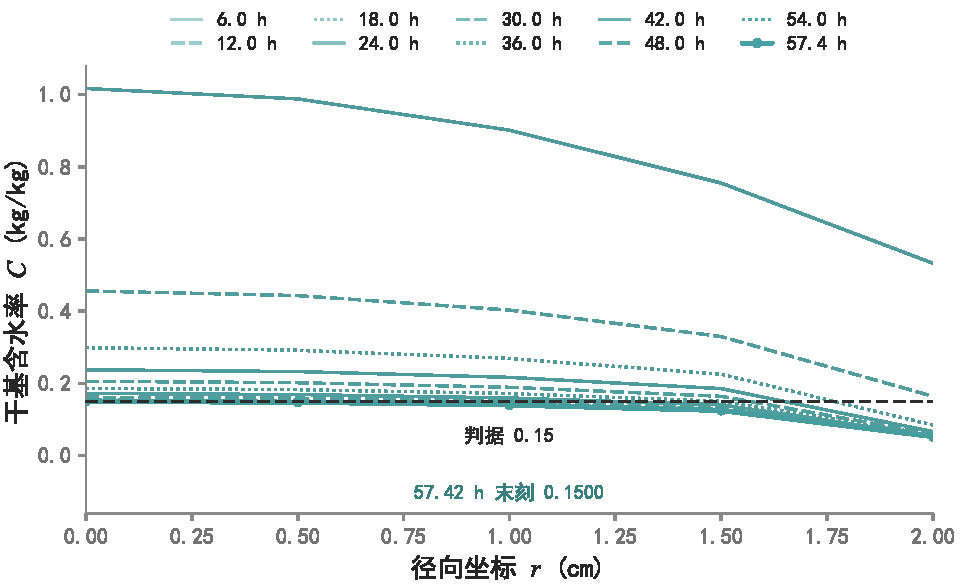
\includegraphics[width=0.9\textwidth,height=0.8\textheight,keepaspectratio]{figures/fig_q3_profiles_6h.pdf}
  \caption{问题三每六小时径向剖面}
  \label{fig:q3_profiles_6h}
\end{figure}

\begin{figure}[H]
  \centering
  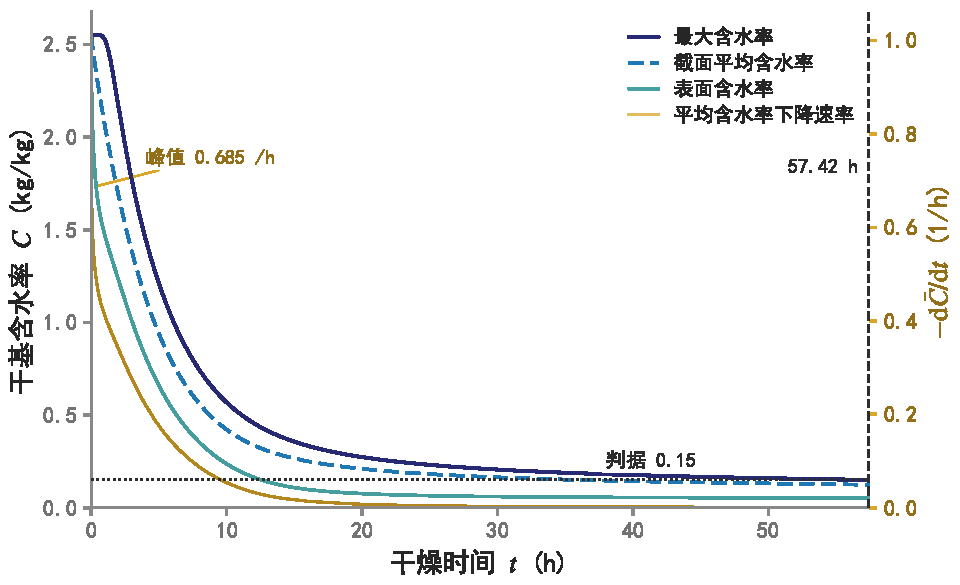
\includegraphics[width=0.9\textwidth,height=0.8\textheight,keepaspectratio]{figures/fig_q3_drying_kinetics.pdf}
  \caption{问题三干燥动力学曲线}
  \label{fig:q3_drying_kinetics}
\end{figure}

% ==== 问题四 ==============================================================
\begin{figure}[H]
  \centering
  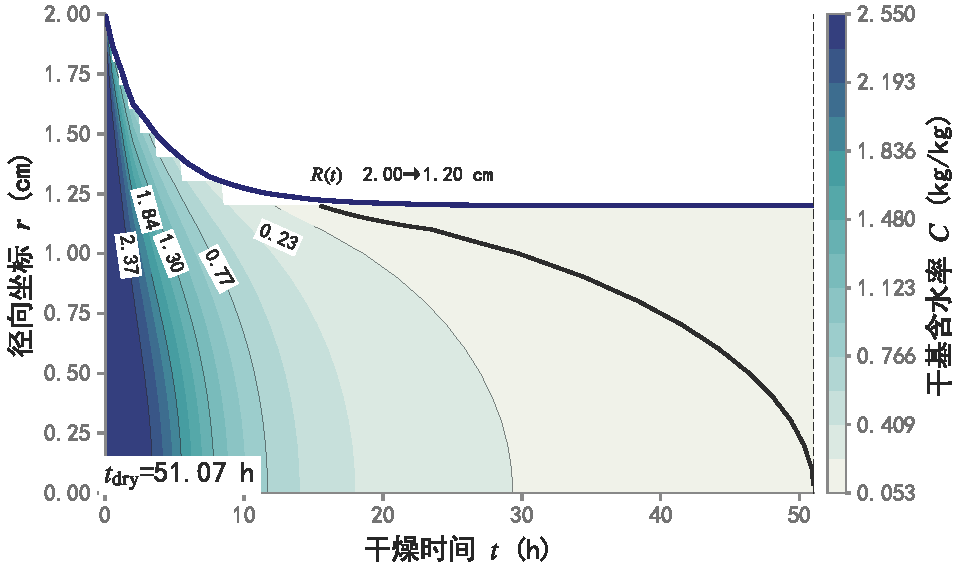
\includegraphics[width=0.9\textwidth,height=0.8\textheight,keepaspectratio]{figures/fig_q4_field_C_moving.pdf}
  \caption{问题四移动边界含水率场}
  \label{fig:q4_field_C_moving}
\end{figure}

\begin{figure}[H]
  \centering
  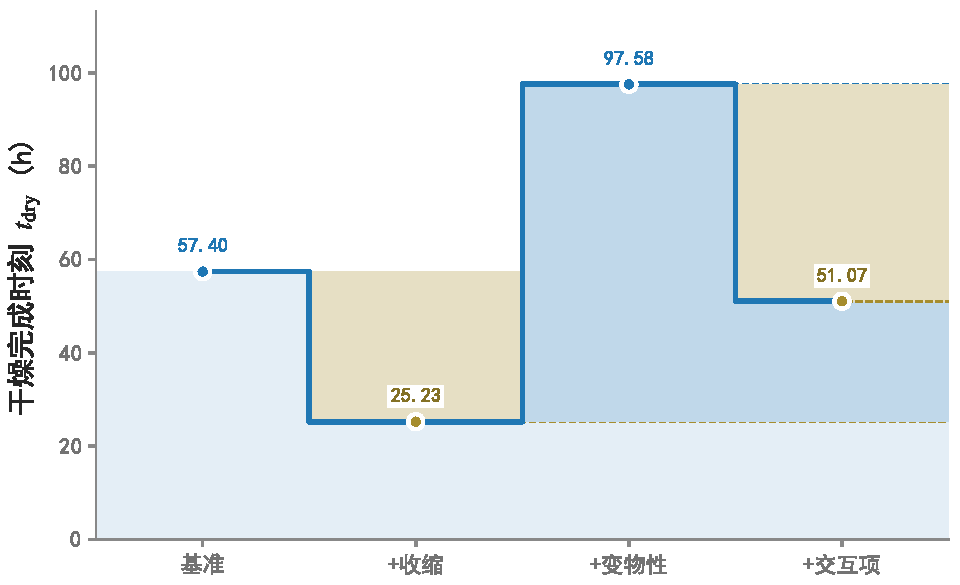
\includegraphics[width=0.9\textwidth,height=0.8\textheight,keepaspectratio]{figures/fig_q4_ablation.pdf}
  \caption{收缩与物性的加性分解}
  \label{fig:q4_ablation}
\end{figure}

% ==== 模型校验与灵敏度 ====================================================
\begin{figure}[H]
  \centering
  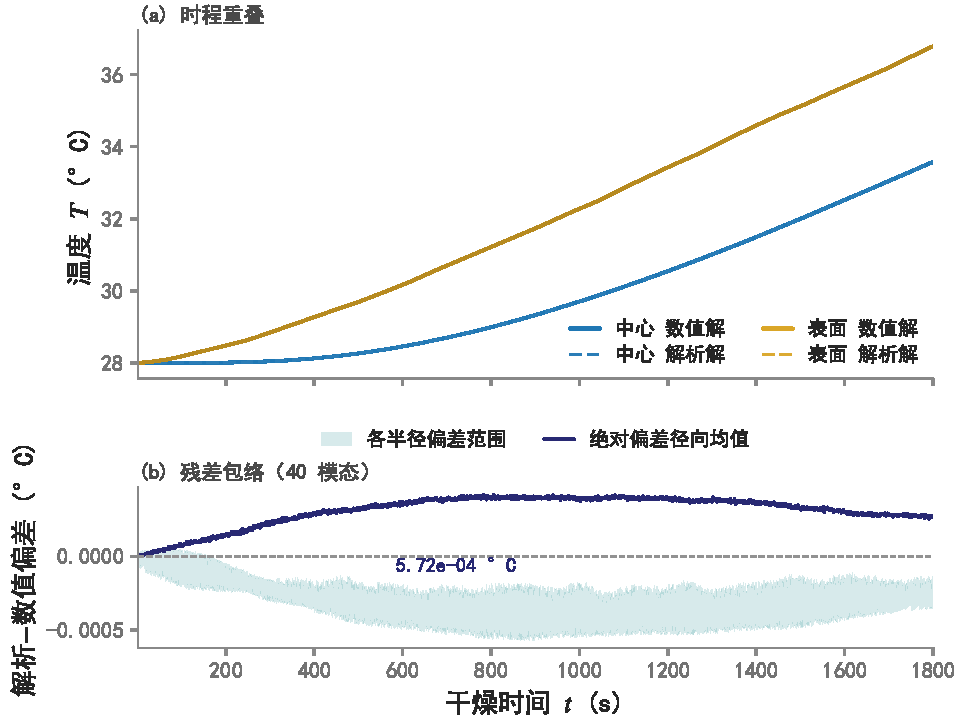
\includegraphics[width=0.9\textwidth,height=0.8\textheight,keepaspectratio]{figures/fig_q1_analytic_val.pdf}
  \caption{解析解与数值解对比}
  \label{fig:q1_analytic_val}
\end{figure}

\begin{figure}[H]
  \centering
  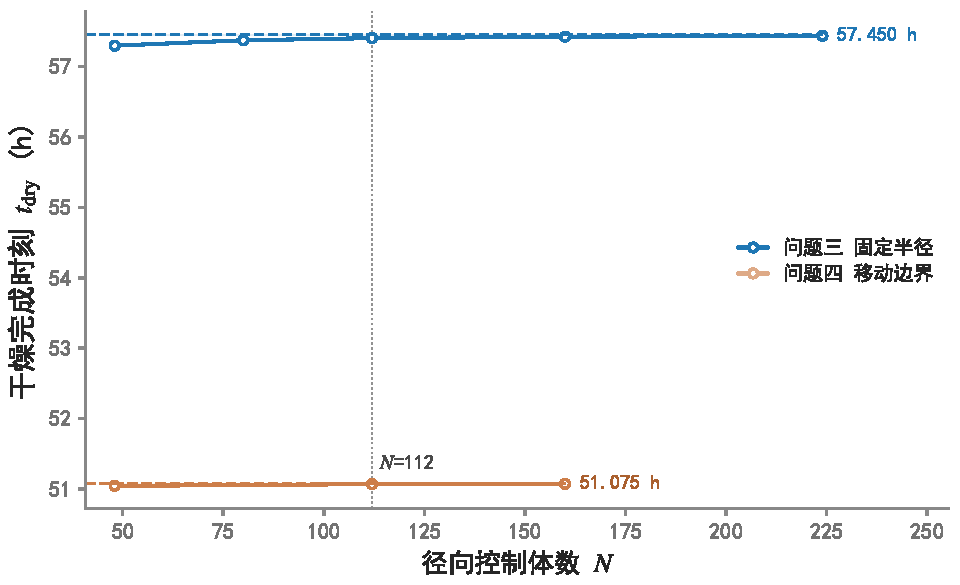
\includegraphics[width=0.9\textwidth,height=0.8\textheight,keepaspectratio]{figures/fig_grid_convergence.pdf}
  \caption{网格收敛性检验}
  \label{fig:grid_convergence}
\end{figure}

\begin{figure}[H]
  \centering
  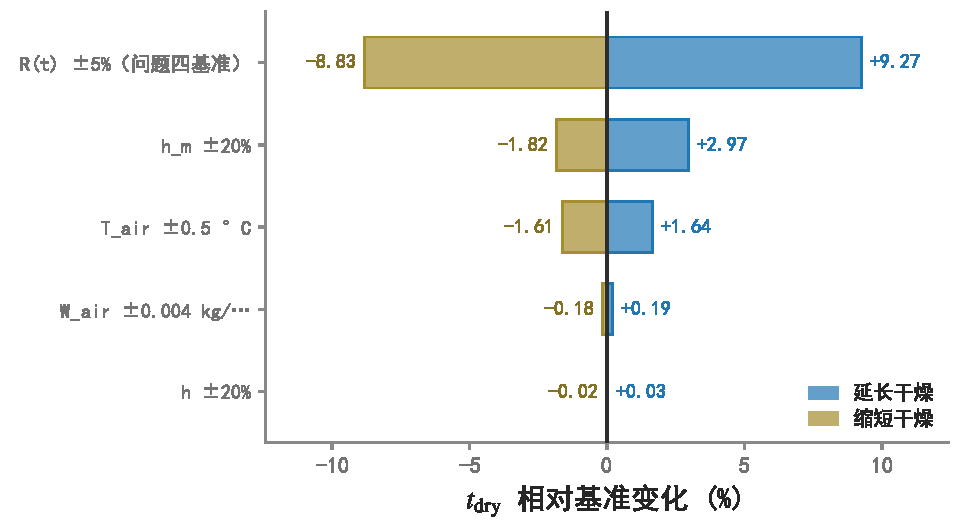
\includegraphics[width=0.9\textwidth,height=0.8\textheight,keepaspectratio]{figures/fig_sensitivity_tornado.pdf}
  \caption{单因子灵敏度排序}
  \label{fig:sensitivity_tornado}
\end{figure}

% ==== 技术路线与问题关系（HTML → 矢量 PDF） ================================
\begin{figure}[H]
  \centering
  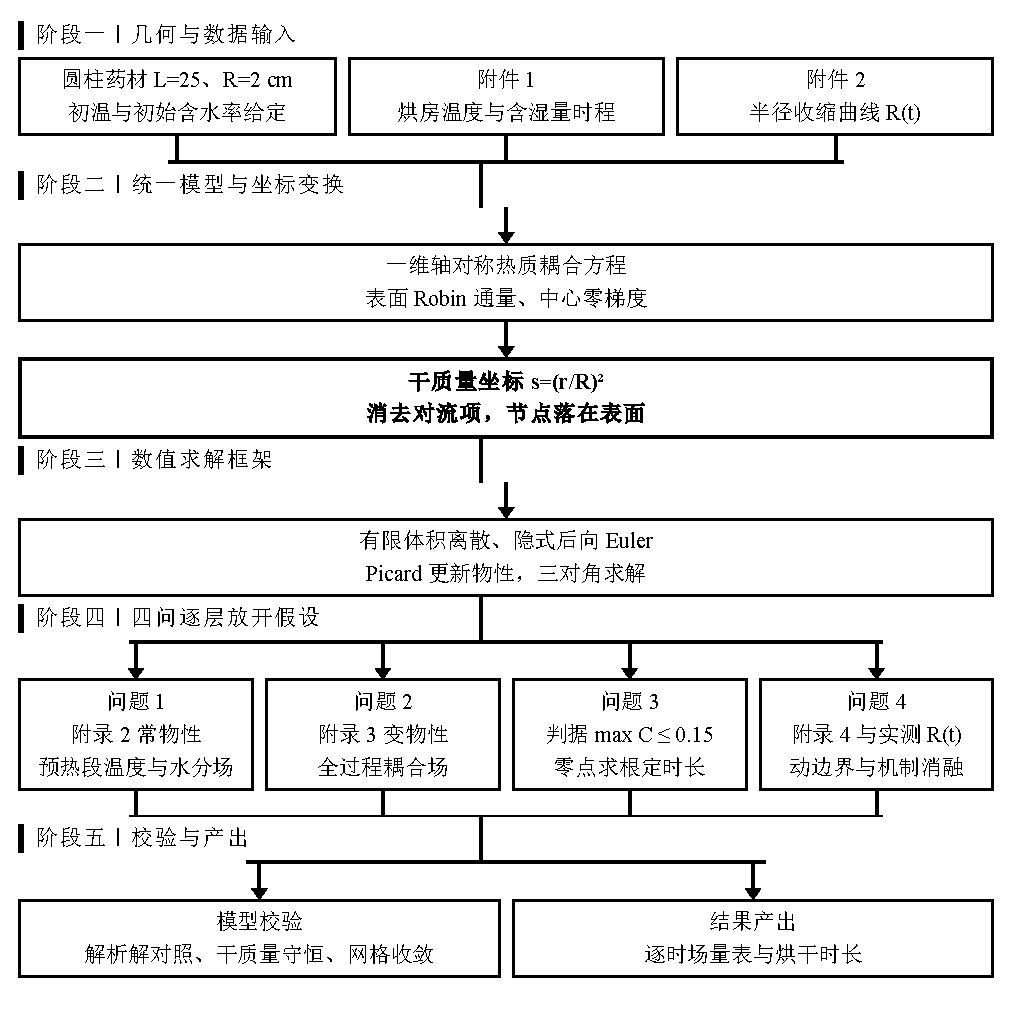
\includegraphics[width=0.94\textwidth,height=0.8\textheight,keepaspectratio]{figures/fig_roadmap_drawio.pdf}
  \caption{整体建模技术路线}
  \label{fig:roadmap}
\end{figure}

\begin{figure}[H]
  \centering
  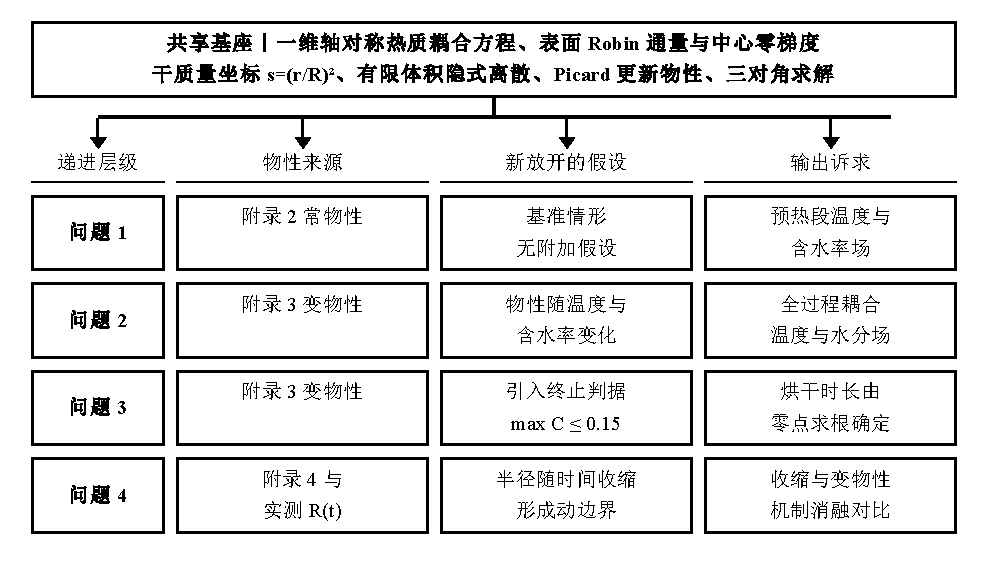
\includegraphics[width=0.9\textwidth,height=0.8\textheight,keepaspectratio]{figures/fig_problem_relation_drawio.pdf}
  \caption{四问关系与递进层次}
  \label{fig:problem_relation}
\end{figure}

% ==== 几何与数值方法示意（TikZ → 矢量 PDF） ================================
\begin{figure}[H]
  \centering
  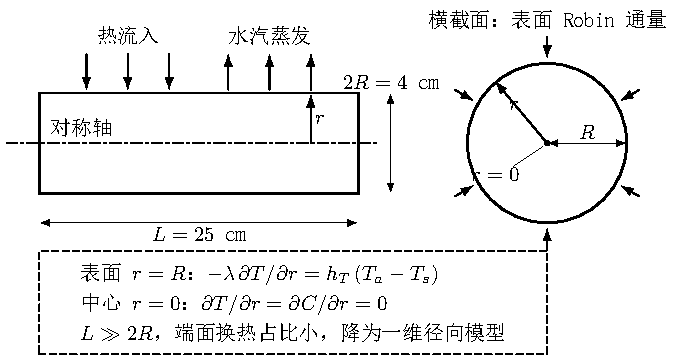
\includegraphics[width=0.9\textwidth,height=0.8\textheight,keepaspectratio]{figures/tikz_cylinder_geometry.pdf}
  \caption{圆柱几何与边界条件}
  \label{fig:cylinder_geometry}
\end{figure}

\begin{figure}[H]
  \centering
  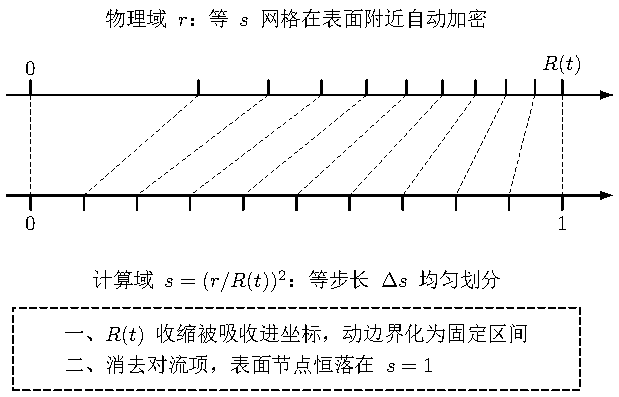
\includegraphics[width=0.9\textwidth,height=0.8\textheight,keepaspectratio]{figures/tikz_coord_mapping.pdf}
  \caption{干质量坐标映射关系}
  \label{fig:coord_mapping}
\end{figure}

\begin{figure}[H]
  \centering
  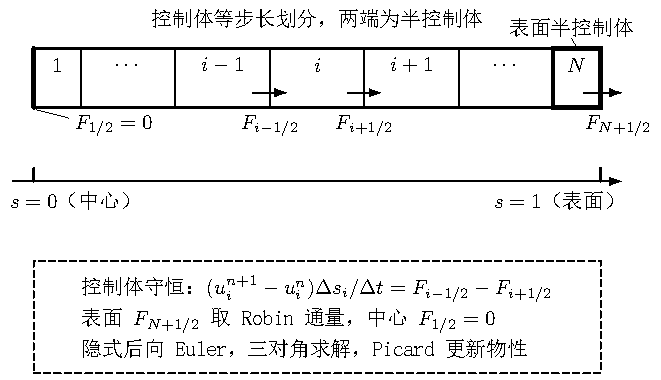
\includegraphics[width=0.9\textwidth,height=0.8\textheight,keepaspectratio]{figures/tikz_fv_stencil.pdf}
  \caption{有限体积控制体与通量}
  \label{fig:fv_stencil}
\end{figure}

% ==== 三线表 ==============================================================
% 13 张表已单独成文件，直接 \input 即可（每张自带 \caption 与 \label）：
%   \begin{table}[H]
  \centering
  \caption{附件输入数据描述性统计}
  \label{tab:input_stats}
  \begin{tabular}{lrrrl}
    \toprule
    输入序列 & 样本数 & 起始或 3 h 值 & 末段值 & 备注 \\
    \midrule
    附件 1 热风温度 (°C) & 241 & 50.1950 & 50.0095 & 13020 s 起 \\
    附件 1 热风含湿量 (kg/kg) & 241 & 0.04977 & 0.04999 & 13020 s 起 \\
    附件 2 药材半径 (cm) & 145 & 2.000 & 1.198 & 6 h 时 1.374 \\
    \bottomrule
  \end{tabular}
  \par\vspace{2pt}\footnotesize 数据来源：figures/problem\_2\_results.json 的 air (.n\_points / .T\_at\_10800 / .W\_at\_10800 / .T\_tail\_mean / .W\_tail\_mean / .tail\_t\_start\_s) 与 figures/problem\_4\_results.json 的 radius\_history (.n\_points / .R0\_cm / .R\_min\_cm / .R\_6h\_cm)。末段值对附件 1 为 tail\_t\_start\_s 之后各点的均值，对附件 2 为全程最小半径。
\end{table}
     % 附件输入数据描述性统计
%   \begin{table}[H]
  \centering
  \caption{问题一药材温度分布}
  \label{tab:q1_T}
  \begin{tabular}{rrrrrr}
    \toprule
    时间 (s) & 0 cm & 0.5 cm & 1 cm & 1.5 cm & 2 cm \\
    \midrule
    100 & 28.0001 & 28.0004 & 28.0041 & 28.0328 & 28.1802 \\
    300 & 28.0410 & 28.0637 & 28.1516 & 28.3683 & 28.8491 \\
    600 & 28.4538 & 28.5364 & 28.8043 & 29.3162 & 30.1655 \\
    900 & 29.3248 & 29.4587 & 29.8759 & 30.6165 & 31.7306 \\
    1200 & 30.5432 & 30.7102 & 31.2228 & 32.1129 & 33.4279 \\
    1500 & 31.9962 & 32.1871 & 32.7664 & 33.7465 & 35.1204 \\
    1800 & 33.5757 & 33.7723 & 34.3644 & 35.3624 & 36.7857 \\
    \bottomrule
  \end{tabular}
  \par\vspace{2pt}\footnotesize 数据来源：figures/problem\_1\_results.json 的 table1\_T；径向位置取同文件 table\_radii\_cm。
\end{table}
            % 问题一药材温度分布
%   \begin{table}[H]
  \centering
  \caption{问题一药材水分浓度}
  \label{tab:q1_C}
  \begin{tabular}{rrrrrr}
    \toprule
    时间 (s) & 0 cm & 0.5 cm & 1 cm & 1.5 cm & 2 cm \\
    \midrule
    100 & 2.5500 & 2.5500 & 2.5500 & 2.5500 & 2.2473 \\
    300 & 2.5500 & 2.5500 & 2.5500 & 2.5492 & 2.0509 \\
    600 & 2.5500 & 2.5500 & 2.5500 & 2.5353 & 1.8770 \\
    900 & 2.5500 & 2.5500 & 2.5497 & 2.5045 & 1.7548 \\
    1200 & 2.5500 & 2.5500 & 2.5482 & 2.4646 & 1.6586 \\
    1500 & 2.5500 & 2.5499 & 2.5445 & 2.4206 & 1.5788 \\
    1800 & 2.5500 & 2.5497 & 2.5383 & 2.3755 & 1.5103 \\
    \bottomrule
  \end{tabular}
  \par\vspace{2pt}\footnotesize 数据来源：figures/problem\_1\_results.json 的 table2\_C；径向位置取同文件 table\_radii\_cm。
\end{table}
            % 问题一药材水分浓度
%   \begin{table}[H]
  \centering
  \caption{问题二药材温度分布}
  \label{tab:q2_T}
  \begin{tabular}{rrrrrr}
    \toprule
    时间 (h) & 0 cm & 0.5 cm & 1 cm & 1.5 cm & 2 cm \\
    \midrule
    0.5 & 32.1900 & 32.3828 & 32.9666 & 33.9614 & 35.4135 \\
    1 & 40.3816 & 40.5536 & 41.0605 & 41.8783 & 42.9977 \\
    1.5 & 45.8464 & 45.9345 & 46.1927 & 46.6048 & 47.1398 \\
    2 & 48.4500 & 48.4878 & 48.5982 & 48.7733 & 49.0032 \\
    2.5 & 49.4668 & 49.4790 & 49.5135 & 49.5653 & 49.6610 \\
    3 & 49.8495 & 49.8553 & 49.8746 & 49.9101 & 49.9664 \\
    \bottomrule
  \end{tabular}
  \par\vspace{2pt}\footnotesize 数据来源：figures/problem\_2\_results.json 的 table3\_T。
\end{table}
            % 问题二药材温度分布
%   \begin{table}[H]
  \centering
  \caption{问题二药材水分浓度}
  \label{tab:q2_C}
  \begin{tabular}{rrrrrr}
    \toprule
    时间 (h) & 0 cm & 0.5 cm & 1 cm & 1.5 cm & 2 cm \\
    \midrule
    0.5 & 2.5499 & 2.5489 & 2.5255 & 2.3257 & 1.6487 \\
    1 & 2.5256 & 2.4948 & 2.3578 & 2.0230 & 1.4711 \\
    1.5 & 2.3860 & 2.3256 & 2.1344 & 1.8020 & 1.3476 \\
    2 & 2.1708 & 2.1084 & 1.9236 & 1.6259 & 1.2311 \\
    2.5 & 1.9567 & 1.9006 & 1.7360 & 1.4720 & 1.1167 \\
    3 & 1.7662 & 1.7165 & 1.5702 & 1.3333 & 1.0081 \\
    \bottomrule
  \end{tabular}
  \par\vspace{2pt}\footnotesize 数据来源：figures/problem\_2\_results.json 的 table4\_C。
\end{table}
            % 问题二药材水分浓度
%   \begin{table}[H]
  \centering
  \caption{问题三烘干过程水分浓度}
  \label{tab:q3_C}
  \begin{tabular}{lrrrrr}
    \toprule
    时间 (h) & 0 cm & 0.5 cm & 1 cm & 1.5 cm & 2 cm \\
    \midrule
    6 & 1.0169 & 0.9881 & 0.9015 & 0.7550 & 0.5328 \\
    12 & 0.4561 & 0.4431 & 0.4030 & 0.3297 & 0.1642 \\
    18 & 0.2988 & 0.2915 & 0.2687 & 0.2253 & 0.0845 \\
    24 & 0.2378 & 0.2327 & 0.2167 & 0.1855 & 0.0665 \\
    30 & 0.2058 & 0.2018 & 0.1891 & 0.1640 & 0.0598 \\
    36 & 0.1858 & 0.1825 & 0.1718 & 0.1503 & 0.0566 \\
    42 & 0.1720 & 0.1691 & 0.1596 & 0.1406 & 0.0548 \\
    48 & 0.1618 & 0.1591 & 0.1506 & 0.1334 & 0.0537 \\
    54 & 0.1538 & 0.1514 & 0.1436 & 0.1276 & 0.0530 \\
    烘干结束 57.4247 & 0.1500 & 0.1477 & 0.1402 & 0.1249 & 0.0526 \\
    \bottomrule
  \end{tabular}
  \par\vspace{2pt}\footnotesize 数据来源：figures/problem\_3\_results.json 的 table5\_C 与 table5\_times\_h；末行时刻为 t\_dry\_h。
\end{table}
            % 问题三烘干过程水分浓度
%   \begin{table}[H]
  \centering
  \caption{问题四烘干过程水分浓度}
  \label{tab:q4_C}
  \begin{tabular}{lrrrrr}
    \toprule
    时间 (h) & 0 cm & 0.5 cm & 1 cm & 药材表面 & $R(t)$ (cm) \\
    \midrule
    6 & 1.7195 & 1.5376 & 1.0226 & 0.4208 & 1.374 \\
    12 & 0.7375 & 0.6545 & 0.4082 & 0.1669 & 1.248 \\
    18 & 0.4086 & 0.3686 & 0.2397 & 0.0892 & 1.214 \\
    24 & 0.2850 & 0.2610 & 0.1789 & 0.0673 & 1.204 \\
    30 & 0.2263 & 0.2093 & 0.1492 & 0.0595 & 1.201 \\
    36 & 0.1928 & 0.1796 & 0.1316 & 0.0559 & 1.200 \\
    42 & 0.1712 & 0.1603 & 0.1199 & 0.0541 & 1.200 \\
    48 & 0.1561 & 0.1468 & 0.1115 & 0.0530 & 1.200 \\
    烘干结束 51.0711 & 0.1500 & 0.1413 & 0.1081 & 0.0526 & 1.200 \\
    \bottomrule
  \end{tabular}
  \par\vspace{2pt}\footnotesize 数据来源：figures/problem\_4\_results.json 的 table6.rows (.C\_fixed / .C\_surface / .R\_cm)；末列表面位置随 $R(t)$ 内移。
\end{table}
            % 问题四烘干过程水分浓度
%   \begin{table}[H]
  \centering
  \caption{四问主结果汇总}
  \label{tab:main_results}
  \begin{tabular}{lllrr}
    \toprule
    问题 & 物性闭合 & 几何 & 时间跨度或 $t_{\mathrm{dry}}$ & 结束时 $\max_r C$ \\
    \midrule
    问题一 & 附录 2 常物性 & 固定 $R$ & 1800 s & -- \\
    问题二 & 附录 3 变物性 & 固定 $R$ & 3 h & -- \\
    问题三 & 附录 3 变物性 & 固定 $R$ & 57.4247 h & 0.1500 \\
    问题四 & 附录 4 变物性 & $R(t)$ 收缩 & 51.0711 h & 0.1500 \\
    \bottomrule
  \end{tabular}
  \par\vspace{2pt}\footnotesize 数据来源：figures/problem\_$k$\_results.json（$k=1,2,3,4$）的 table\_times\_s / table\_times\_h / t\_dry\_h / C\_max\_at\_end；问题一、二为指定时间跨度，不涉及干燥判据。
\end{table}
    % 四问主结果汇总
%   \begin{table}[H]
  \centering
  \caption{问题四消融实验}
  \label{tab:ablation}
  \begin{tabular}{lrr}
    \toprule
    工况组合 & $t_{\mathrm{dry}}$ (h) & 相对基准 (\%) \\
    \midrule
    固定半径 + 附录 3（问题三基准） & 57.4040 & 0.0000 \\
    收缩 + 附录 3 基准物性 & 25.2269 & -56.0538 \\
    固定半径 + 换附录 4 物性 & 129.7587 & 126.0445 \\
    收缩 + 附录 4（完整） & 51.0671 & -11.0393 \\
    \bottomrule
  \end{tabular}
  \par\vspace{2pt}\footnotesize 数据来源：figures/problem\_4\_results.json 的 ablation (.baseline\_h / .shrink\_only\_h / .props\_only\_h / .full\_h 与对应 \_pct)；交互项 -46.5145 h 为四者的加性分解残差，亦取自同字段 .interaction\_h。
\end{table}
        % 问题四消融实验
%   \begin{table}[H]
  \centering
  \caption{单因子灵敏度汇总}
  \label{tab:sensitivity}
  \begin{tabular}{lrr}
    \toprule
    扰动工况 & $t_{\mathrm{dry}}$ (h) & 相对基准 (\%) \\
    \midrule
    基准（问题三） & 57.4040 & 0.0000 \\
    $T_{\mathrm{air}}$+0.5 °C & 56.4813 & -1.6075 \\
    $T_{\mathrm{air}}$-0.5 °C & 58.3477 & 1.6439 \\
    $W_{\mathrm{air}}$+0.004 kg/kg & 57.5144 & 0.1923 \\
    $W_{\mathrm{air}}$-0.004 kg/kg & 57.3029 & -0.1762 \\
    $h_m$ $\times$1.2 & 56.3565 & -1.8249 \\
    $h_m$ $\times$0.8 & 59.1107 & 2.9730 \\
    h $\times$1.2 & 57.3910 & -0.0227 \\
    h $\times$0.8 & 57.4238 & 0.0343 \\
    $R(t)$ $\times$1.05（基准问题四） & 55.8023 & 9.2725 \\
    $R(t)$ $\times$0.95（基准问题四） & 46.5590 & -8.8277 \\
    \bottomrule
  \end{tabular}
  \par\vspace{2pt}\footnotesize 数据来源：figures/sensitivity\_results.json 的 rows (.label / .t\_dry\_h / .rel\_pct)；每行均按 meta.recompute=full\_simulation\_per\_row 全程重算。末两行以问题四为基准（baseline\_q4\_h=51.0671 h），其余以问题三为基准（baseline\_q3\_h=57.4040 h）。
\end{table}
     % 单因子灵敏度汇总
%   \begin{table}[H]
  \centering
  \caption{问题三网格收敛性}
  \label{tab:grid}
  \begin{tabular}{rrr}
    \toprule
    径向控制体数 $N$ & $t_{\mathrm{dry}}$ (h) & 相对前一档差 (\%) \\
    \midrule
    48 & 57.2968 & -- \\
    80 & 57.3738 & 0.1343 \\
    112 & 57.4040 & 0.0527 \\
    160 & 57.4247 & 0.0360 \\
    224 & 57.4370 & 0.0214 \\
    \bottomrule
  \end{tabular}
  \par\vspace{2pt}\footnotesize 数据来源：figures/problem\_3\_results.json 的 grid\_convergence (.N / .t\_dry\_h / .rel\_diff)；百分比列为 rel\_diff 乘 100。
\end{table}
            % 问题三网格收敛性
%   \begin{table}[H]
  \centering
  \caption{问题三时间步收敛性}
  \label{tab:dt}
  \begin{tabular}{rr}
    \toprule
    时间步 $\Delta t$ (s) & $t_{\mathrm{dry}}$ (h) \\
    \midrule
    4.0 & 57.4067 \\
    2.0 & 57.4049 \\
    1.0 & 57.4040 \\
    0.5 & 57.4036 \\
    \bottomrule
  \end{tabular}
  \par\vspace{2pt}\footnotesize 数据来源：figures/problem\_3\_results.json 的 dt\_convergence (.dt\_s / .t\_dry\_h)，径向控制体数固定为 112。
\end{table}
              % 问题三时间步收敛性
%   \begin{table}[H]
  \centering
  \caption{各问干质量守恒残差}
  \label{tab:conservation}
  \begin{tabular}{lr}
    \toprule
    算例 & 相对残差 \\
    \midrule
    问题一 & 4.218e-11 \\
    问题二 & 2.139e-11 \\
    问题三 & 3.425e-10 \\
    问题四 & 1.547e-10 \\
    \bottomrule
  \end{tabular}
  \par\vspace{2pt}\footnotesize 数据来源：figures/problem\_$k$\_results.json 的 conservation\_residual（$k=1,2,3,4$）。
\end{table}
    % 各问干质量守恒残差
